\subsection{Studies in the Uniform Phase Space} % (fold)
\label{sub:flat_hypercube_studies}

An important part of the investigation into what the neutral networks are learning beyond the standard physics features is to quantify the performance when these features are removed.  One way to remove the discrimination power from a given feature is to apply a transformation such that the marginal likelihood ratio is constant at unity.  In other words, we derive event-by-event weights such that

\begin{equation}
\label{eq:flat}
  f(m, \tau_{21}, p_T| W'\rightarrow WZ) \approx f(m, \tau_{21}, p_T| QCD).
\end{equation}

Figure~\ref{fig:rocCube} shows the ROC curve for various features with this weighting scheme applied.  By construction, $\tau_{21}$ and the jet mass do not have any discrimination power between signal and background, evident by the fact that $\epsilon_\text{bkg}=\epsilon_\text{signal}$.    However, the convolutional network that is trained inclusively does have some discrimination power.  For a fixed signal efficiency, the overall performance is significantly degraded with respect to the un-weighted ROC curve in Fig.~\ref{fig:combinedROC1}, but the improvement over a random guess is significant.  Interestingly, the `other' information learned by the network is effectively gathered during the inclusive training - there is only a marginal improvement by performing a dedicated training of the convolution network with the weights applied.

\begin{figure}[htbp]
  \centering
  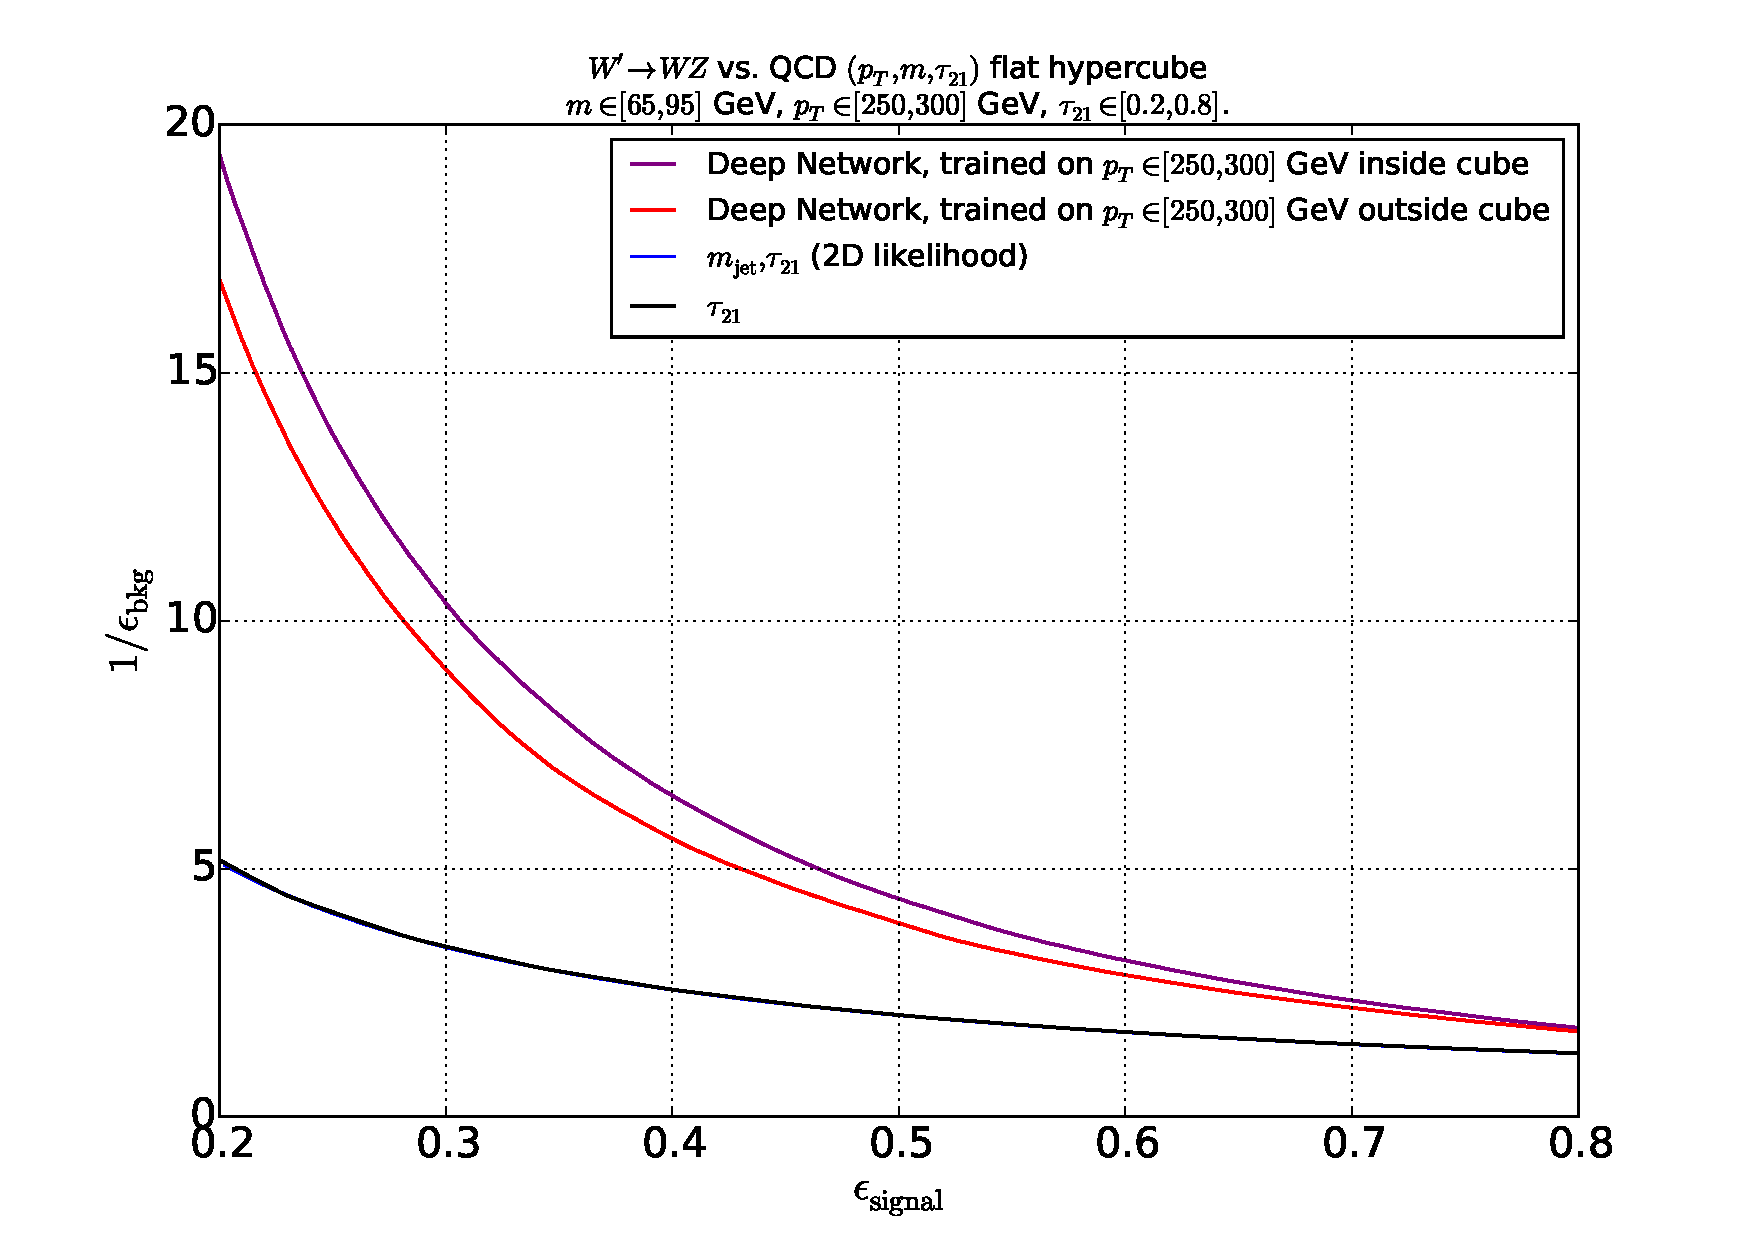
\includegraphics[width=0.95\textwidth]{figures/roc-cube-inside.pdf}
  \caption{Various ROC curves with event weights that enforce Eq.~\ref{eq:flat} inside $m\in[65, 95]\mathsf{GeV}$,  $p_T\in[250, 300]\mathsf{GeV}$, and  $\tau_{21}\in[0.2, 0.8]$.  By construction, the $\tau_{21}$ and likelihood combination of $\tau_{21}$ and mass are non-discriminating.  The Deep Network lines are for the convolution network without normalization and using the energy-scheme for pixel intensities.  One network is trained without weights ({\it outside}) and one is trained with the weights applied ({\it inside}).}
  \label{fig:rocCube}
\end{figure}


\begin{figure}[htbp]
  \centering
  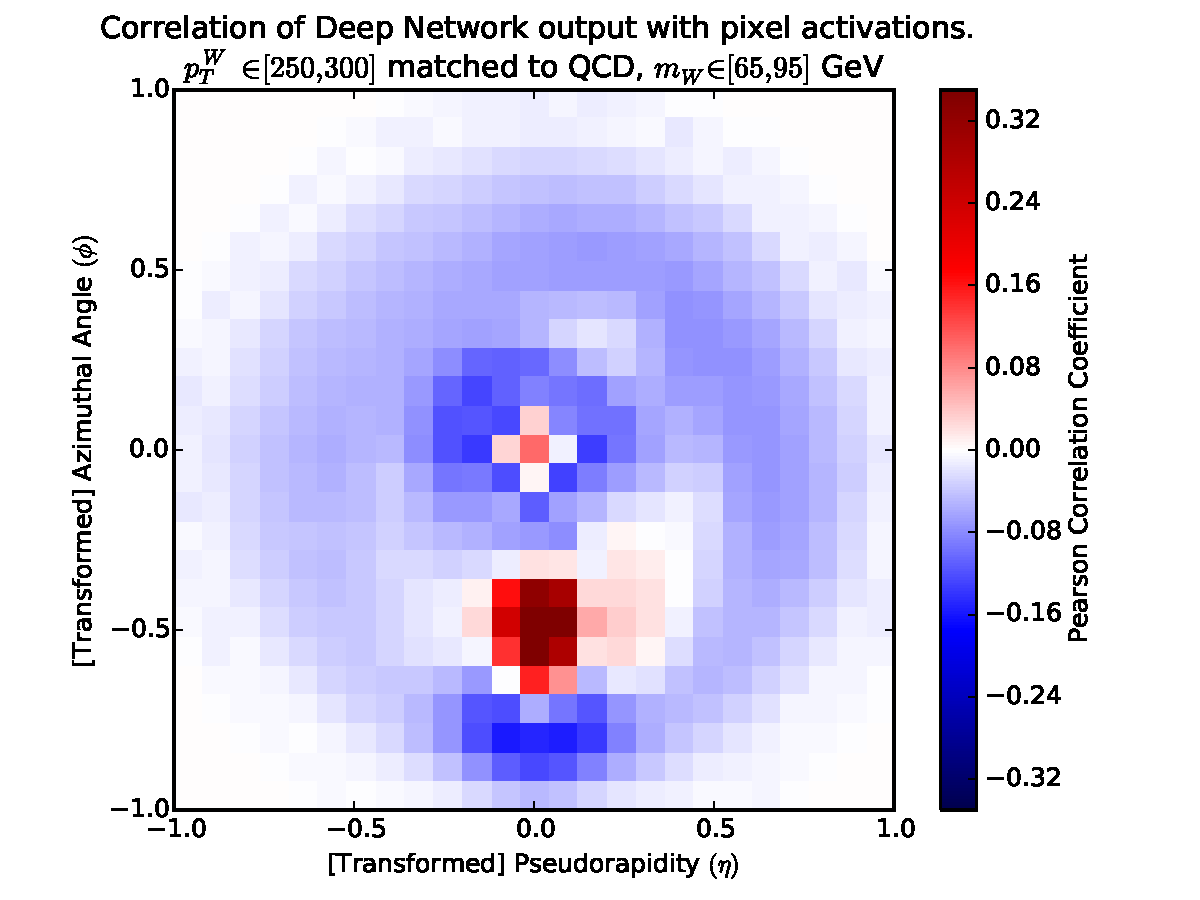
\includegraphics[width=0.45\textwidth]{figures/hypercube-pixel-activations-corr.pdf} 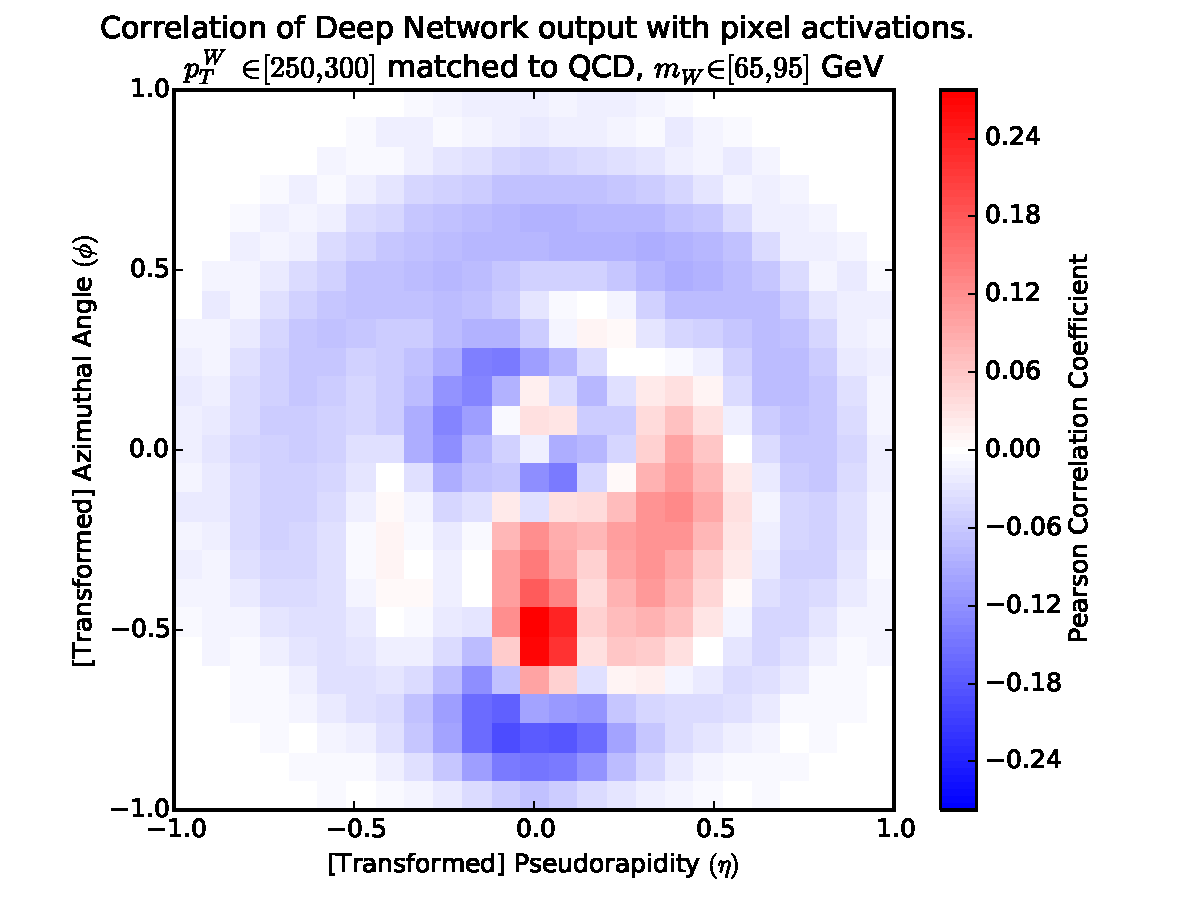
\includegraphics[width=0.45\textwidth]{figures/ahypercube-pixel-activations-corr.pdf}
  \caption{Left: trained inclusively but weighted for the plot and right is trained with uniform weights and also weighted for the plot.}
  \label{fig:images_hyper}
\end{figure}

% subsection flat_hypercube_studies (end)